\documentclass[../Thesis.tex]{subfiles}
\begin{document}
	
	\section{State of the Art Review}
	\label{sec:state_of_the_art_review}
	
	Calculating the GED with traditional imperative algorithm is possible but feasible for graphs of modest size. GED is a NP-HARD problems and for traditional solutions there is no way except to compare graphs node by node and edge by edge through combinatorial techniques to find a solution. However, as the number of nodes in the graphs increase, the complexity of these methods grows exponentially, leading to scalability issues thus infeasibility. To overcome these limitations recent works involve the use of artificial intelligence techniques such as neural networks to predict the GED between two graphs. AI-based approaches usually offer more robust and scalable solutions by learning patterns and features from graphs, significantly reducing computation times. This section reviews some of the most important papers dealing with GED calculation from 2019 to the time of writing this (2024).

	The timeline we are going to explore starts with \textit{SimGNN} in 2019 \cite{simgnn__a_neural_network_approach_to_fast_graph_similarity_computation}, the first prominent approach to utilize neural networks for computing GED. 
	After that many other models have been built mostly on SimGNN's foundation each time trying to perform a little better.
	Finally the timeline ends with most recent and promising work introducing \textit{GedGNN} \cite{computing_graph_edit_distance_via_neural_graph_matching}. All these models try to effectively predict the GED between two graphs, but as we will see, everything seems still to be in early stage of development.
	
	\subsection{Timeline}
	\label{subsec:timeline}
	
	2019, \textit{SimGNN: A Neural Network Approach to Fast Graph Similarity Computation} \cite{simgnn__a_neural_network_approach_to_fast_graph_similarity_computation}: Introduces SimGNN, addressing graph similarity computation using neural networks. It features a learnable embedding function, an attention mechanism to focus on important nodes, and a pairwise node comparison method, achieving better generalization and computational efficiency compared to baselines.
	
	2020, \textit{Learning Graph Edit Distance by Graph Neural Networks} \cite{learning_graph_edit_distance_by_graph_neural_networks}: Introduces a framework combining deep metric learning with traditional approximations of graph edit distance using geometric deep learning. The approach employs a message passing neural network (MPNN) to capture graph structure and compute graph distances efficiently, showing superior performance in graph retrieval and competitive results in graph similarity learning.
	
	2020, \textit{Combinatorial Learning of Graph Edit Distance via Dynamic Embedding} \cite{combinatorial_learning_of_graph_edit_distance_via_dynamic_embedding}: Introduces a hybrid approach for solving the GED problem by integrating a dynamic graph embedding network with an edit path search procedure, enhancing interpretability and cost-efficiency. The learning-based A* algorithm reduces search tree size and saves time with minimal accuracy loss.
	
	2021, \textit{Graph Partitioning and Graph Neural Network-Based Hierarchical Graph Matching for Graph Similarity Computation} \cite{graph_partitioning_and_graph_neural_network_based_hierarchical_graph_matching_for_graph_similarity_computation}: Introduces PSimGNN, which partitions input graphs into subgraphs to extract local structural features, then uses a novel GNN with attention to map subgraphs to embeddings, combining coarse-grained interaction among subgraphs with fine-grained node-level comparison to predict similarity scores.
	
	2021, \textit{Noah: Neural Optimized A* Search Algorithm for Graph Edit Distance Computation} \cite{noah__neural_optimized_a*_search_algorithm_for_graph_edit_distance_computation}: Introduces Noah, combining A* search algorithm and Graph Path Networks (GPN) for approximate GED computation. Noah learns an estimated cost function using GPN, incorporates pre-training with attention-based information, and adapts an elastic beam size to reduce search complexity.
	
	2021, \textit{Learning Efficient Hash Codes for Fast Graph-Based Data Similarity Retrieval} \cite{learning_efficient_hash_codes_for_fast_graph_based_data_similarity_retrieval}: Introduces HGNN (Hash Graph Neural Network), a model designed for efficient graph-based data retrieval by leveraging GNNs and hash learning algorithms. HGNN learns a similarity-preserving graph representation and computes compact hash codes for fast retrieval and classification tasks.
	
	2021, \textit{More Interpretable Graph Similarity Computation via Maximum Common Subgraph Inference} \cite{more_interpretable_graph_similarity_computation_via_maximum_common_subgraph_inference}: Introduces INFMCS, an interpretable end-to-end paradigm for graph similarity learning, leveraging the correlation between similarity score and Maximum Common Subgraph (MCS), combining transformer encoder layers with graph convolution for superior performance and interpretability.
	
	2021, \textit{H2MN: Graph Similarity Learning with Hierarchical Hypergraph Matching Networks} \cite{h2mn__graph_similarity_learning_with_hierarchical_hypergraph_matching_networks}: Introduces H2MN, which measures similarities between graph-structured objects by transforming graphs into hypergraphs and performing subgraph matching at the hyperedge level, followed by a multi-perspective cross-graph matching layer.
	
	2022, \textit{TaGSim: Type-aware Graph Similarity Learning and Computation} \cite{TaGSim_type_aware_graph_similarity_learning_and_computation}: Proposes TaGSim, a framework that addresses the limitations of traditional GED methods by incorporating type-specific graph edit operations. TaGSim models the transformative impacts of different graph edits (node and edge insertions, deletions, and relabelings) separately, creating type-aware embeddings and using these embeddings for accurate GED estimation. The framework demonstrates superior performance on real-world datasets compared to existing GED solutions.
	
	2023, \textit{Efficient Graph Edit Distance Computation Using Isomorphic Vertices} \cite{efficient_graph_edit_distance_computation_using_isomorphic_vertices}: Proposes a novel approach for reducing the search space of GED computation by leveraging isomorphic vertices, targeting redundant vertex mappings and significantly cutting computation costs for exact GED.
	
	2023, \textit{Exploring Attention Mechanism for Graph Similarity Learning} \cite{exploring_attention_mechanism_for_graph_similarity_learning}: Proposes a unified framework with attention mechanisms, combining graph convolution and self-attention for node embedding, cross-graph co-attention for interaction modeling, and graph similarity matrix learning for score prediction, showing superior performance on benchmark datasets.
	
	2023, \textit{Graph Edit Distance Learning via Different Attention} \cite{graph_edit_distance_learning_via_different_attention}: Introduces DiffAtt, a novel graph-level fusion module for GNNs to compute GED efficiently by leveraging graph structural differences using attention mechanisms, incorporated into the GSC model REDRAFT, achieving state-of-the-art performance on benchmark datasets.
	
	2023, \textit{Graph-Graph Context Dependency Attention for Graph Edit Distance} \cite{graph_graph_context_dependency_attention_for_graph_edit_distance}: Introduces GED-CDA, a deep network architecture for GED computation that incorporates a graph-graph context dependency attention module, leveraging cross-attention and self-attention layers to capture inter-graph and intra-graph dependencies.
	
	2023, \textit{GREED: A Neural Framework for Learning Graph Distance Functions} \cite{greed__a_neural_framework_for_learning_graph_distance_functions}: Introduces GREED, a siamese GNN designed to learn GED and Subgraph Edit Distance (SED) in a property-preserving manner, achieving superior accuracy and efficiency compared to state-of-the-art methods.
	
	2023, \textit{MATA*: Combining Learnable Node Matching with A* Algorithm for Approximate Graph Edit Distance} \cite{mata_combining_learnable_node_matching_with_a*_algorithm_for_approximate_graph_edit_distance}: Introduces MATA*, a hybrid approach for approximate GED computation leveraging GNNs and A* algorithms, focusing on learning to match nodes rather than directly regressing GED.
	
	2023, \textit{Multilevel Graph Matching Networks for Deep Graph Similarity Learning} \cite{multilevel_graph_matching_networks_for_deep_graph_similarity_learning}: Proposes MGMN, a multilevel graph matching network capturing cross-level interactions, comprising a Node-Graph Matching Network (NGMN) and a siamese GNN for global-level interactions, demonstrating superior performance as graph sizes increase.
	
	2023, \textit{Wasserstein Graph Distance Based on L1-Approximated Tree Edit Distance Between Weisfeiler-Lehman Subtrees} \cite{wasserstein_graph_distance_based_on_l1_approximated_tree_edit_distance_between_weisfeiler_lehman_subtrees}: Proposes the WWLS distance, combining WL subtrees with L1-approximated tree edit distance (L1-TED), capable of detecting subtle structural variations in graphs, demonstrating superiority in metric validation and graph classification tasks.
	
	
	2023, \textit{Computing Graph Edit Distance via Neural Graph Matching} \cite{computing_graph_edit_distance_via_neural_graph_matching}: Introduces GEDGNN, a deep learning framework for computing GED by focusing on graph conversion rather than GED value prediction alone. GEDGNN predicts GED values and a matching matrix, followed by a post-processing algorithm for extracting high-quality node matchings.
	
	\subsection{SimGNN}
	
	The first innovative model that used neural networks is SimGNN \cite{simgnn__a_neural_network_approach_to_fast_graph_similarity_computation}, introduced in 2019. SimGNN serves as a foundational model in the field of graph similarity computation, in fact future models will often inherit its core concepts (such as the siamese layout architecture), making it the starting point of reference for anyone dealing with GED computation. 
	
	The architecture of SimGNN [\autoref{fig:simgnn_architecture}] is composed by several stages:
	
	\begin{itemize}
		\item \textbf{Node Embedding Stage}: This stage makes use of a graph convolutional network to capture local structural information that transforms each node in the graph into a vector that encodes its features and structural properties.
		\item \textbf{Graph-Level Embedding Stage}: This stage produces a single embedding representing the whole graphs starting from the previously produced nodes embeddings by also using attention mechanisms to focus on important nodes.
		\item \textbf{Graph-Graph Interaction Stage}: This stage puts in communication the two graphs embedding previously produced and produces a matrix of similarity interaction scores.
		\item \textbf{Final Similarity Score Computation Stage}: This stage process the previously produced similarity matrix to compute the final similarity score.
	\end{itemize}
	
	In addition to the graph-level embedding interaction strategy, SimGNN has a its disposal a pairwise node comparison strategy:
	
	\begin{itemize}
		\item \textbf{Pairwise Node Comparison}: This strategy involves computing pairwise interaction scores between the node embeddings of the two graphs. The resulting similarity matrix is used to extract histogram features, which are then combined with the graph-level interaction scores to provide a comprehensive view of graph similarity.
	\end{itemize}
	
	The combination of these two strategies should allow the model to capture both global and local informations which should result in a robust approach to graph similarity computation.
	
	\begin{figure}[H]
		\centering
		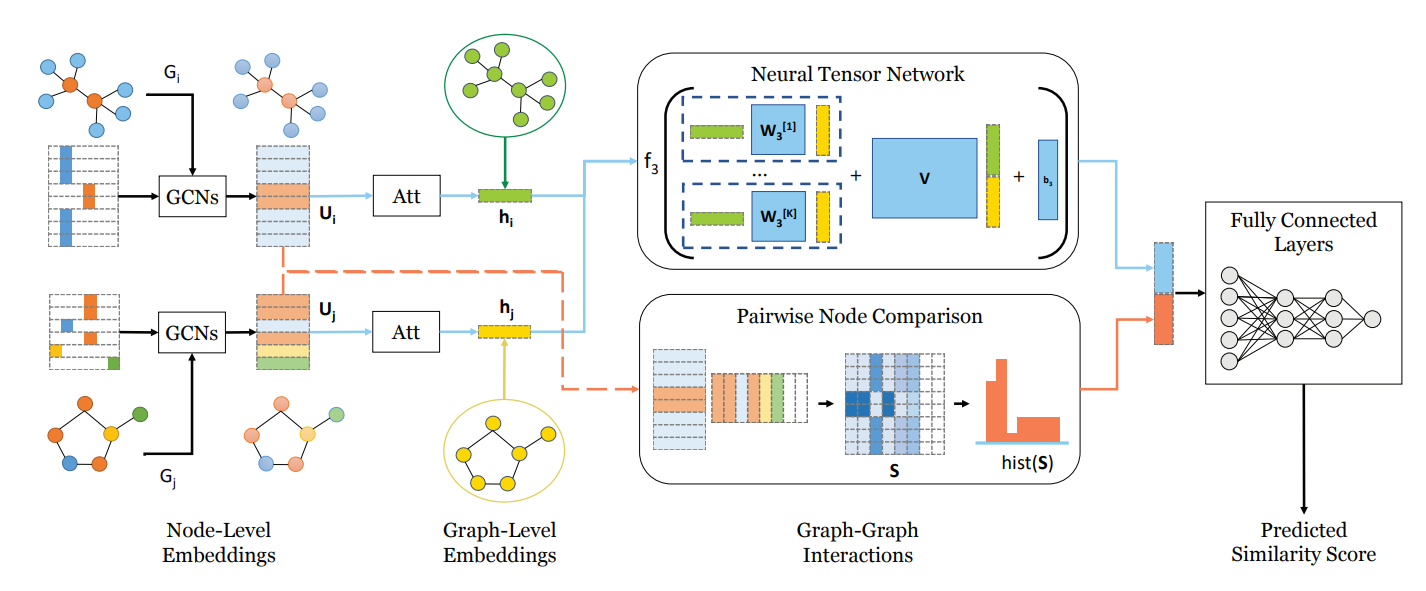
\includegraphics[width=\textwidth]{Images/simgnn_architecture.png}
		\caption{SimGNN architecture overview.}
		\label{fig:simgnn_architecture}
	\end{figure}

	
	\subsection{GPN}
	
	In 2022, an innovative hybrid approach for computing GED was released.
	The Graph Path Networks (GPN) model, proposed within the \textit{NOAH Framework} \cite{noah__neural_optimized_a*_search_algorithm_for_graph_edit_distance_computation}, introduces the GED computation by exploiting the A* search algorithm optimized through neural networks. This method tries to address several previously found limitations trying to improve both the search direction and search space optimization.
	
	The architecture of GPN [\autoref{fig:gpn_architecture}] is composed by several modules:
	
	\begin{itemize}
		\item \textbf{Pre-training Module}: This module computes pre-training information about the graphs that will be exploited by the next modules.
		\item \textbf{Graph Embedding Module}: This module utilizes layers of Graph Isomorphism Network (GIN) to transform each node into a vector. Then these embeddings are combined into a single graph level embedding by using different attention mechanisms.
		\item \textbf{Learning Module}: This module focuses on optimizing the A* search algorithm by learning an estimated cost function and an elastic beam size. The tradition algorithm is then used for the final prediction.
	\end{itemize}
	
	The main advantage of GPN over SimGNN is that it is capable of finding an edit path between graphs (roughly accurate) between graphs in a short amount of time.
	
	\begin{figure}[H]
		\centering
		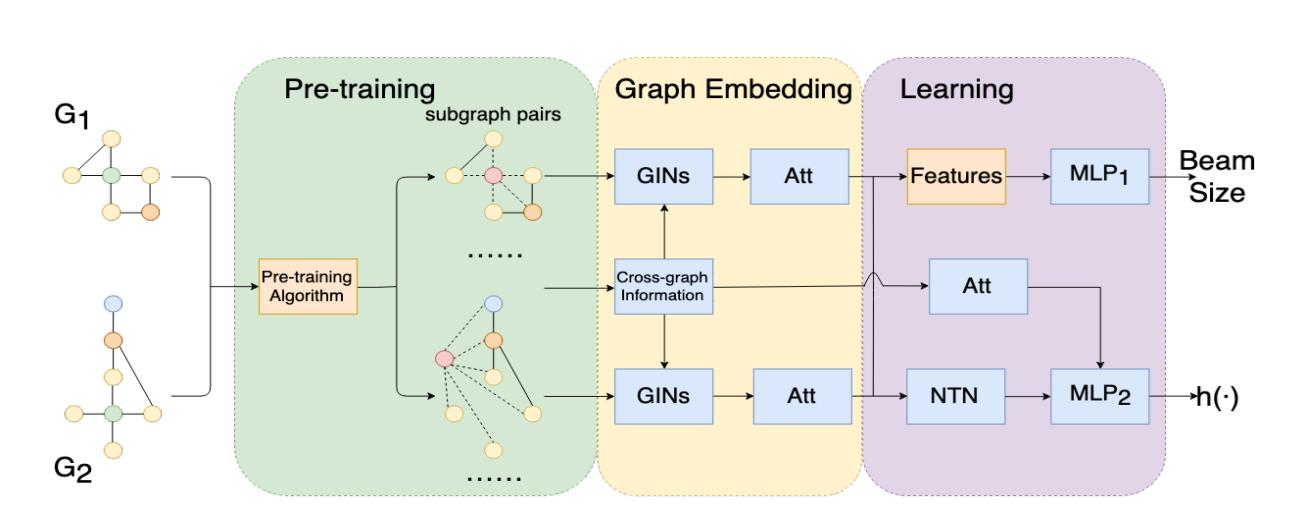
\includegraphics[width=\textwidth]{Images/gpn_architecture.png}
		\caption{GPN architecture overview.}
		\label{fig:gpn_architecture}
	\end{figure}
	
	
	\subsection{TaGSim}
	
	In 2022, another innovative approach was released with TaGSim (Type-aware Graph Similarity) \cite{TaGSim_type_aware_graph_similarity_learning_and_computation}. The idea behind GED as a single value has been revaluated and it is now thought as the summation of three different values: $ged\_nc$ the number of node relabelling, $ged\_in$ the number of node insertions/deletions, $ged\_ie$ the number of edges insertions/deletions. 
	
	The architecture of TaGSim [\autoref{fig:tagsim_architecture}] is composed by several components:
	
	\begin{itemize}
		\item \textbf{Type-Aware Graph Embeddings}: This component takes into account the different impacts that different atomic operations could have when predicting the GED producing a type-aware graph level embedding. Namely the operations taken into accounts are: node insertion/deletion (NR), node relabeling (NID), edge insertion/deletion (ER), and edge relabeling (EID). Each type of operation is handled separately to capture its localized effects on the graph.
		\item \textbf{Type-Aware Neural Networks}: This component takes advantage of specific neural networks that are specifically designed to process and learn from the type-aware embeddings. This allows TaGSim to achieve high accuracy in GED estimation by incorporating the distinct impacts of different edit types and outputs them all.
	\end{itemize}
	
	The main advantage of TaGSim over predecessors is that by decoupling the GED into different dimensions, there is the potential for more granular control and learnability.
	
	\begin{figure}[H]
		\centering
		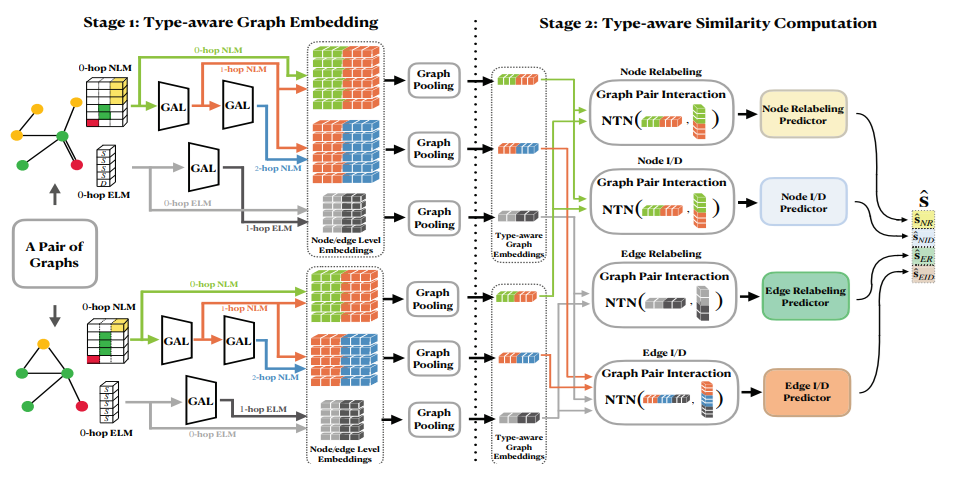
\includegraphics[width=\textwidth]{Images/tagsim_architecture.png}
		\caption{TaGSim architecture overview.}
		\label{fig:tagsim_architecture}
	\end{figure}

	\subsection{GedGNN}
	
	In 2023, the model that is considered the state of the art at the time of writing this (2024) is released with GedGNN (Graph Edit Distance via Neural Graph Matching) \cite{computing_graph_edit_distance_via_neural_graph_matching}. The idea behind this model is to try to put together all the best ideas from past's models including the basic siamese layout of SimGNN, the use of more advanced convolutional layers of GPN and the split of the GED metric from TaGSim while still allowing for the retrieval of an edit paths by taking inspiration from NOAH framework.
	
	The architecture of GedGNN [\autoref{fig:gedgnn_architecture}] is composed by several components:
	
	\begin{itemize}
		\item \textbf{Graph Neural Network (GNN) Encoder}: This component produces the encodings for nodes and edges while preserving their relational information. This is done through the employment of an advanced GNN encoder.
		\item \textbf{Node and Edge Matching Module}: This component performs the node and edge matching between the pair of graphs producing a matching matrix and a cost matrix.
		\item \textbf{k-Best Matching Post-Processing Algorithm}: After predicting the GED value a k-best post-processing algorithm is used trying to retrieve a good edit path.
	\end{itemize}
	
	GedGNN's results state to not only outperforms previous methods but also provides a flexible framework that can adapt to various types of graph structures and similarity measures.
	
	\begin{figure}[H]
		\centering
		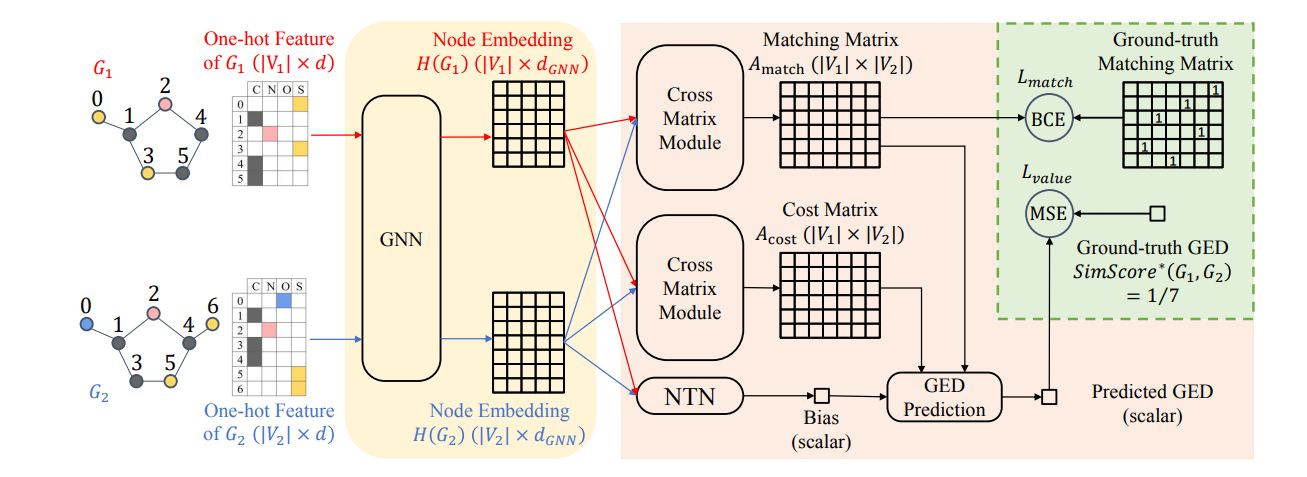
\includegraphics[width=\textwidth]{Images/gedgnn_architecture.png}
		\caption{GedGNN architecture overview.}
		\label{fig:gedgnn_architecture}
	\end{figure}
	
	\subsection{Encountered Gaps}
	
	When studying GedGNN's \href{https://github.com/ChengzhiPiao/GEDGNN}{codebase} a lot of problems and concerns have become evident. Perhaps most of these gaps are due to the intrinsic nature of copy pasting from paper to paper over time and to the lack of researcher's ability to extensively testing theyr work.
	
	A primary issue is the quality of the codebase itself, there is a lack of standardization and employments of best practices, lots of similar methods that all seem to do the same thing, lots of classes, lots of confusion, lots of unhandled errors. Code almost seem hardcoded here and there, not allowing for customization and manipulation. The code is not easy to read and the documentation, although written, is very poor.
	
	Strictly correlated to code quality and testing scenarios is the scalability issues on GPUs. When trying to run for the first time the code as is on a GPU some errors also raised up, but apart from this, the models do not scale well on GPU hardware and this is an issue. Training on small datasets is feasible on CPUs but as soon as a bigger dataset are used for test-training new models, problems have become evident with long training times per epoch.
	
	It is not clear why the codebase as is does restrict the usage of graphs for those with only 10 nodes or less in both training, testing and validation scenarios. Perhaps due to the presence of many imperative algorithm with high computational time such as the k-best post processing algorithm that retrieves edit paths; also code as is does break (at least for me) when testing on the IMDB dataset (with any model). Additionally, there is no use of artificial dataset generation, despite being present in the code, creating more confusion and several if statements that will never be reached.
	
	Data used for training is also an issue persisting from SimGNN's times. Datasets used are always the same but the issue (which is not an issue but rather a constructive critic), is that approximate GEDs are used as labels instead of real ones. Datasets are mostly small (with graphs with less than 10 nodes in general) and with modern hardware GED wouldn't take much time to compute exactly. Also, in almost any codebase seen till date, training is structured in such a way that for each pair of graph present in the training set the corresponding GED is required.
	
	But the most important thing that has been shown up is that testing has not been performed in a fair way. It is not clear why, but when dealing with the codebase as is, it is not possible to test a model that has been trained on a specific dataset on a different dataset. Perhaps to not show the evident lack of generalization emersed after doing modifications to the code to perform fair testing [\autoref{sec:methodology_and_experimentation}].
	
	In summary, the analysed codebase which presents GedGNN, TaGSim, SimGNN and GPN presents several significant challenges to overcome. These include problems with the reproducibility of the results, fair evaluations, scalability issues, poor code quality, unclear parameters and more. Clearly, resolving many of this issues would lead to a significant advancement in this field.
	
\end{document}
